\begin{warpHTML}
\begin{wrapfigure}{r}{0.5\textwidth}
  \begin{center}
    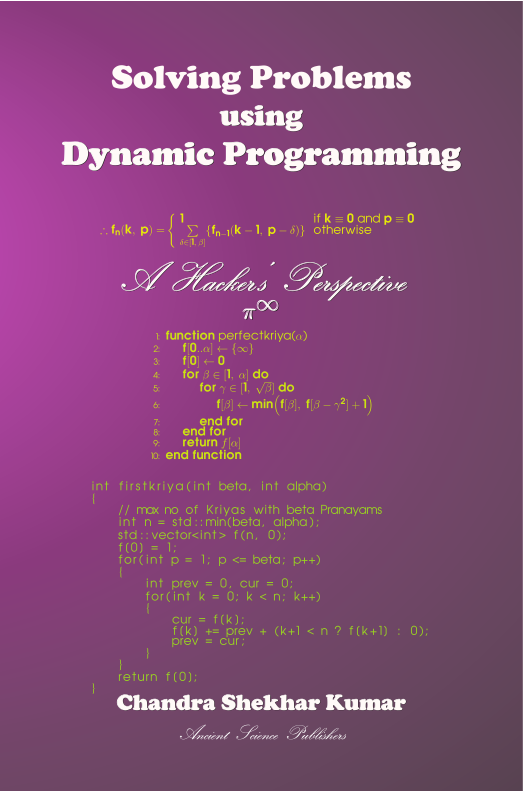
\includegraphics[width=0.5\textwidth]{solvingdpp/cover/dpp-cover}
  \end{center}
  %\caption{Front Cover}
\end{wrapfigure}
\end{warpHTML}

\hspace{5mm}A hacker's approach to a coding problem is beyond the foundational aspect of underlying genetic and computational structures, often termed as $\color{Orange}\mathbf{\pi^\infty}$.  

\begin{warpprint}
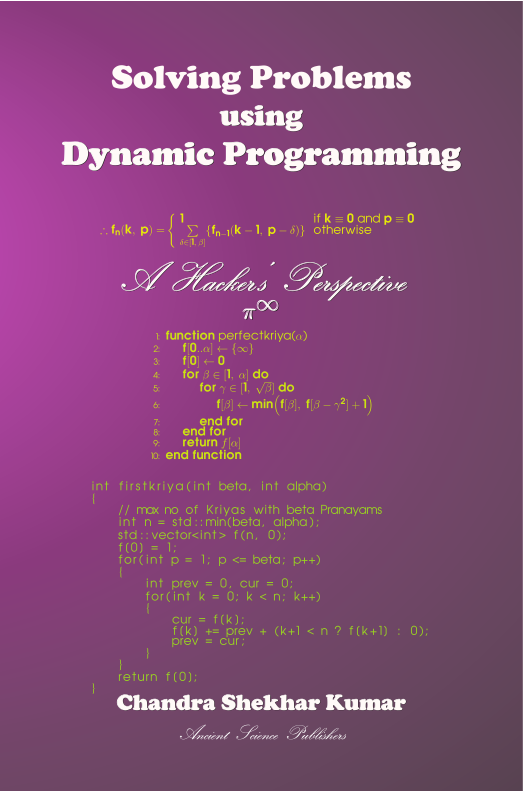
\includegraphics[width=0.5\linewidth]{solvingdpp/cover/dpp-cover}
\end{warpprint}

\hspace{5mm}A concept becomes \hlt{not difficult} because the \hlt{complexities} built into it are clarified. In a bid to reach the \hlt{core} of the problem, the concept is split-broken into fragments,  \hlt{complexities} are exposed and \hlt{delicate} points are examined. Then the concept is \hlt{recomposed} to make it integral and as a result, this reintegrated concept becomes sufficiently simple and comprehensible. 

\hspace{5mm}This helps build a hacker's insight to reveal the internal structure and internal logic of the concepts, algorithms and mathematical theorems.

\vspace{3mm}

This book provides a hacker's perspective to solving problems using dynamic programming. Written in an extremely lively form of problems and solutions (including code in modern C++ and pseudo style), this leads to extreme simplification of optimal coding with great emphasis on unconventional and integrated science of dynamic Programming. Though aimed primarily at serious programmers, it imparts the knowledge of deep internals of underlying concepts and beyond to computer scientists alike.


\vspace{0.2in}

\noindent {\calligra Ancient Science Publishers}  \hfill \emph{Chandra Shekhar Kumar}

\noindent July, 2020. \hfill 256 pages \hfill ISBN  9781722497170

\vspace{5mm}

\begin{quote}
\hspace{5mm}\hlt{Beautiful (C++) code snippets. Unique yogic exposition to coding.}
\end{quote}
\hfill {\calligra Ancient Science Hackers}


\vspace{10mm}


\underline{\textbf{\textcolor{BurntOrange}{Excerpt from the Chapter} \textcolor{Sepia}{(Optimal Loot Partition):}}}


\begin{p}
\hlt{The head of a gang of robbers embarks on distribution of the looted amount $l (> 0)$, starting with division into two parts : $x$ and $l - x$ for $0 \le x \le l$. From $x$ : they get a return of $u(x)$ such that they are left with a lesser amount $\alpha x$ : $0 < \alpha < 1$ and from $l - x$ : a return of $v(l - x)$ such that they are left with a lesser amount $\beta(l - x)$ : $0 < \beta < 1$. So the total amount left after the first step of division is $\alpha x + \beta (l - x)$ and the process continues. Devise the partition strategy to help them maximize the return obtained in a finite $n$ or infinite number of steps.}
\end{p}

\begin{s}
Let $y(x)$ denote the return after the first step:
\begin{gather*}
\therefore y(x) = u(x) + v(l - x)
\end{gather*}
Assuming $u$ and $v$ to be continuous functions, it is trivial to find the maximum of $y(x)$ over $x \in [0, l]$ using calculus (or graphical approach) :
\begin{gather*}
\dfrac{d y}{d x} = \dfrac{d}{d x} u(x) + \dfrac{d}{d x} v(l - x) = 0 \text{ (for extrema)}.
\end{gather*}
Solve for $x$ and $y(x)$ is maximum for that $x$ for which $\dfrac{d^2 y}{d x^2} < 0$.

Suppose $u(x) = x$ and $v(l - x) = -(l - x)^2 $, then 
\begin{gather*}
y = x - (l - x)^2 \\
\therefore \dfrac{d y}{d x} = 1 + 2(l - x) = 0, \\
\therefore x = l + \dfrac{1}{2}.\\
\dfrac{d^2 y}{d x^2} = -2 < 0. \\
\therefore y_{max} = l + \dfrac{1}{2} - \dfrac{1}{4} = l + \dfrac{1}{4}. 
\end{gather*}
After the first step, the initial amount $l$ is reduced to $l_1$(say):
\begin{gather*}
\therefore l_1 = \alpha x + \beta (l - x) 
\end{gather*}
In the second step, $l_1$ is partitioned into $x_1$ (say) and $(l_1 - x_1)$ for $0 \le x_1 \le l_1$. Hence, the return from the second step is $u(x_1) + v(l_1 - x_1)$. Therefore, the total return after the two steps is:
\begin{gather*}
\therefore y(x, x_1) = u(x) + v(l - x) + u(x_1) + v(l_1 - x_1).
\end{gather*}
Maximum of the function $y(x, x_1)$ over the 2-dimensional space $(x, x_1)$ yields the maximum return, such that $x \in [0, l]$ and $x_1 \in [0, l_1]$.

Similarly, the total return after $n$ steps is :
\begin{gather}
\therefore y(x, x_1, x_2, \ldots, x_{n - 1}) = u(x) + v(l - x) + \sum_{i=1}^{n - 1}\left[u(x_i) + v(l_i - x_i)\right].
\end{gather}

Here $x_i \in [0, l_i]$.

\vspace{2mm}

Using this \emph{enumerative} approach to maximize the $n$-dimen-sional return, the computation procedure soon becomes cumbersome, error-prone and exponential in nature. 

\vspace{2mm}

Any choice of $x, x_1, x_2, \ldots$ is a \emph{policy}.

The policy maximizing $y(x, x_1, x_2, \ldots)$ is an \emph{optimal policy}.

\vspace{2mm}

It can be noted that each step depends on the respective policy only. Hence at the $(i + 1)^{th}$ step, the corresponding \emph{one-dimensional} choice is made : a choice of $x_i \in [0, l]$.

\vspace{2 mm}

Hence an optimal policy leads to the corresponding maximum return.

Let $y_n (l)$ denote the maximum total return, given the initial amount $l$ and n steps.
\begin{gather*}
\therefore y_1 (l) =  \Max\limits_{x \in [0, l]} \left[u(x) + v(l - x)\right].
\end{gather*}
After the first step, $l$ becomes $\alpha x + \beta (l - x)$ :
\begin{gather*}
\therefore y_2 (l) = \Max\limits_{x \in [0, l]} \left[u(x) + v(l - x) + y_1\left(\alpha x + \beta (l - x)\right) \right].
\end{gather*}
This leads to a recurrence relation :
\begin{gather}
\therefore y_n (l) = \Max\limits_{x \in [0, l]} \left[u(x) + v(l - x) + y_{n - 1} \left(\alpha x + \beta (l - x)\right) \right] . \label{lootpartition:e1}
\end{gather}

Hence a single $n$-dimensional problem is reduced to a sequence of $n$ one-dimensional problems.

Here, the optimal return depends on the initial amount $l$ and initial decision of division into the parts $l$ and $l - x$ only.

\vspace{2 mm}

This is possible due to \hlbt{the Principle of Optimality} : 
\begin{quote}
\hlt{An optimal policy has the property that whatever the initial state and initial decision are, the remaining decisions must constitute an optimal policy with regard to the state resulting from the first decision.}
\end{quote}
Hence~\cref{lootpartition:e1} is the required optimal strategy.
%\par \vspace{-1.9\baselineskip}
%\qedhere
\end{s}




\vspace{15mm}


\underline{\textbf{\textcolor{BurntOrange}{Excerpt from the Chapter} \textcolor{Sepia}{(Constrained Subsequence):}}}


\section*{Maximum Sum}\index{Constrained Subsequence!Maximum Sum}
\begin{p} \label{maxsubarray : sum}\index{Max Sum Subarray}
Given a sequence of $n \in (-\infty, \; \infty)$ integers, determine the largest possible sum of the contiguous subsequence.
\end{p}

\begin{s}
Let $f_n(i)$ be the maximum sum of a contiguous subsequence ending at index $i$, obtained using an optimal policy and $n$ steps.

Let $s_i$ be the value of the element at index $i$, i.e. $s_i$ is used at the $n^{th}$ step. The we can use an optimal policy starting with previously accumulated maximum sum of a contiguous subsequence ending at index $i-1$.

Hence the required optimal procedure is
\begin{align*}
\therefore f_n(i) &= \Max\limits_{i \in [0, \; n-1]} \left[f_{n-1}(i-1) + s_i\right]
\end{align*}

At each step (with addition of $s_i$), there are 2 options :
\begin{enumerate}
    \item leverage the previous accumulated maximum sum if \\$f_{n-1}(i-1) + s_i > 0$, because it is better to continue with a positive running sum or
    \item start afresh with a new range (with the starting sum as 0) if $f_{n-1}(i-1) + s_i < 0$, because it is better to start with 0 than continuing with a negative running sum. 
\end{enumerate} 

Also note that:
\begin{itemize}
    \item If all the elements are negative, then there is no such subsequence, i.e. the required sum is 0.
    \item If all the elements are positive, then the entire sequence is the required subsequence, i.e. the required sum is the sum of all the elements of the sequence.  
    \item The required subsequence (if any) starts at and ends with a positive value.
\end{itemize}



\begin{figure}
\begin{center}
\fbox{\hlbt{Maximum sum contiguous subsequence : compute sum}}
\end{center}
\begin{algorithmic}[1]
\Function{maxseq}{$s[0..n-1]$}
    \State $currentsum \gets 0$
    \State $maxsum \gets 0$
    \For{$x \in s[0 .. n-1]$}
        \State $currentsum \gets$ \textbf{max}$(currentsum + x, 0)$
        \State $maxsum \gets$ \textbf{max}$(maxsum, currentsum)$ 
    \EndFor
    \State \textbf{return} $maxsum$
\EndFunction
\end{algorithmic}
\end{figure}

Time complexity is $\bigO(n)$. Space complexity is $\bigO(1)$.

\begin{lstlisting}
int maxseq(std::vector<int> & s)
{
    int current_sum = 0;
    int max_sum = 0;

    for(int x : s)
    {
        current_sum = std::max(current_sum + x, 0);
        max_sum = std::max(max_sum, current_sum);
    }
    return max_sum;
}
\end{lstlisting}
\par \vspace{-1.2\baselineskip}
\qedhere
\end{s}


\section*{Circular Sequence}\index{Constrained Subsequence!Circular Sequence}

\begin{p}\label{maxcircular:p1}
Given a circular sequence $s$ of $n \in (-\infty, \infty)$ integers, find the maximum possible sum of a non-empty contiguous subsequence of $s$.
\end{p}

\begin{s}
The end of a circular sequence wraps around the start of the sequence itself, i.e.
\begin{gather*}
\because i \equiv (i + n) \; \mathbf{mod} \; n \quad \forall i \in [0, n) \\
\therefore s_i \equiv s_{(i+n) \; \mathbf{mod} \; n} \quad \forall i \in [0, n).
\end{gather*}

\begin{center}
\begin{tikzpicture} %[nodes in empty cells,
      %nodes={minimum width=0.5cm, minimum height=0.5cm},
      %row sep=-\pgflinewidth, column sep=-\pgflinewidth]
      %border/.style={draw}
    
      \matrix(vector)[matrix of nodes, row sep=0.2cm, column sep=-\pgflinewidth, nodes={draw, minimum width=11mm, minimum height=5mm}] (m)
      {
          $s_{0}$ & $s_{1}$ & $\ldots$ & $s_{i}$ & $\ldots$ & $s_{n-1}$\\
          $s_{n}$ & $s_{n+1}$ & $\ldots$ & $s_{n+i}$ & $\ldots$ & $s_{2n-1}$\\
      };
      \foreach \i in {1,...,6}
      {
          \draw[->] (m-2-\i) -- (m-1-\i);
       }
\end{tikzpicture}
\end{center}

For a maximum contiguous subsequence $\mleft[s_i \cdots s_j\mright]$, the solution of~\cref{maxsubarray : sum} can be used.

\begin{center}
\begin{tikzpicture}[
    MyStyle/.style={draw, minimum width=2em, minimum height=2em, 
                outer sep=0pt},
  ]

\matrix (A) [matrix of math nodes, nodes={MyStyle, anchor=center}, column sep=-\pgflinewidth]
{s_0 & \cdots & s_i & s_{i+1} & \cdots & s_{j-1} & s_j & \cdots & s_{n-1}\\};

\draw[decorate,decoration={brace, amplitude=10pt, raise=2pt, mirror}]
  (A-1-3.south west) to node[black,midway,below= 10pt] {max subsequence} (A-1-7.south east);%
\end{tikzpicture}
\end{center}

For a maximum contiguous subsequence $\mleft[s_j \cdots s_{n-1}, s_0 \cdots s_i\mright]$, the left-over part $\mleft[s_{i+1} \cdots s_{j-1}\mright]$ forms a minimum contiguous subsequence.\index{Min Sum Circular Subarray}

\begin{center}
\begin{tikzpicture}[
    MyStyle/.style={draw, minimum width=2em, minimum height=2em, 
                outer sep=0pt},
  ]

\matrix (A) [matrix of math nodes, nodes={MyStyle, anchor=center}, column sep=-\pgflinewidth]
{s_0 & \cdots & s_i & s_{i+1} & \cdots & s_{j-1} & s_j & \cdots & s_{n-1}\\};

\draw[decorate,decoration={brace, amplitude=10pt, raise=2pt, mirror}]
  (A-1-1.south west) to node[black,midway,below= 10pt] {\scriptsize max subseq part 2} (A-1-3.south east);%
\draw[decorate,decoration={brace, amplitude=10pt, raise=2pt, mirror}]
  (A-1-7.south west) to node[black,midway,below= 10pt] {\scriptsize max subseq part 1} (A-1-9.south east);%
  
  \draw[decorate,decoration={brace, amplitude=10pt, raise=2pt, mirror}]
  (A-1-6.north east) to node[black,midway,above= 10pt] {\scriptsize min subsequence} (A-1-4.north west);%
\end{tikzpicture}
\end{center}

Summation of the contiguous subsequence \\$\mleft[s_j \cdots s_{n-1}, s_0 \cdots s_i\mright]$ is
\begin{align*}
&= s_j + \cdots + s_{n-1} + s_0 + \cdots + s_i \\
&= s_0 + \cdots + s_{n-1} - \mleft[s_{i+1} + \cdots + s_{j-1} \mright]
\end{align*}
This is maximum when $\mleft[s_{i+1} + \cdots + s_{j-1} \mright]$ is minimum.
\begin{gather*}
\therefore \Max \mleft[s_j + \cdots + s_{n-1} + s_0 + \cdots + s_i\mright] = \sum\limits_{k=0}^{k=n-1} s_k - \Min \sum\limits_{k=i+1}^{k=j-1} s_k \\
\therefore \text{Maximum sum subsequence } = \text{ Total sum of the sequence } \\
\quad\quad\quad\qq{}\qq{}\qq{} \qq{}\qq{}\qq{} - \text{ Minimum sum subsequence}
\end{gather*}


\begin{figure}
\begin{center}
\fbox{\hlbt{Maximum sum circular subsequence}}
\end{center}
\begin{algorithmic}[1]
\Function{maxcircularseq}{$s[0..n-1]$}
    \State $currentmax \gets 0$
    \State $maxsum \gets -\infty$
    \State $currentmin \gets 0$
    \State $minsum \gets \infty$
    \State $totalsum \gets 0$
    \Statex
    \For{$x \in s[0 .. n-1]$}
        \State $currentmax \gets$ \textbf{max}$(currentmax + x, x)$
        \State $maxsum \gets$ \textbf{max}$(maxsum, currentmax)$ 
        \Statex
        \State $currentmin \gets$ \textbf{min}$(currentmin + x, x)$
        \State $minsum \gets$ \textbf{min}$(minsum, currentmin)$ 
        \Statex
        \State $totalsum \gets totalsum + x$
    \EndFor
    \Statex
    \If{$totalsum == minsum$} \Comment{All elements are -ve}
        \State \textbf{return} $maxsum$ \Comment{Value of the least -ve element}
    \Else
        \State \textbf{return} \textbf{max}$(maxsum, \; totalsum - minsum)$
    \EndIf
\EndFunction
\end{algorithmic}
\end{figure}

Time complexity is $\bigO(n)$. Space complexity is $\bigO(1)$.

\begin{lstlisting}
int maxsum_circular(std::vector<int> & s)
{
    int current_max = 0, max_sum = std::numeric_limits<int>::min();
    int current_min = 0, min_sum = std::numeric_limits<int>::max();
    int total_sum = 0;

    for(int x : s)
    {
        current_max = std::max(current_max + x, x);
        max_sum = std::max(max_sum, current_max);

        current_min = std::min(current_min + x, x);
        min_sum = std::min(min_sum, current_min);

        total_sum += x;
    }
    // when all elements are -ve => total_sum == min_sum, 
    // i.e. total_sum - min_sum becomes 0 => empty subsequence
    // but max_sum still holds the value of the least -ve element,
    // hence return this singleton than an empty one
    return total_sum == min_sum ? max_sum : std::max(max_sum, total_sum - min_sum);
}
\end{lstlisting}

\begin{comment}
\begin{center}
\scalebox{0.9}{
\begin{tabular}{ccc} \hline
\textbf{Circular Sequence} & \textbf{Max Sum Subsequence} & \textbf{Max Sum} \\ \hline
1,-2,3,-2 & 3 & 3\\ \hline
5,3,-5 & 5,5 & 10 \\ \hline
3,-1,2,-1 & 3,-1,2 and 2, -1, 3 & 4 \\ \hline
3,-2,2,-3 & 3 and 3,-2,2 & 3 \\ \hline
-2,-3,-1 & -1 & -1 \\ \hline
8,-1,3,4 & 3,4,8 & 15 \\ \hline
5,-3,5,5,-3 & 5,-3,5,5 and 5,5,-3,5 & 12 \\ \hline
\end{tabular}}
\end{center}
\par\vspace{-0.5\baselineskip}
\qedhere
\end{comment}
\end{s}


\section*{Brief Table of Contents}

\begin{enumerate}[noitemsep]
\item Genesis
    \begin{enumerate}
        \item Optimal Loot Partition
         \begin{enumerate}
             \item Deterministic
             \item Stochastic
         \end{enumerate}
        \item Exam Prep
        \item Optimal Coin Tossing
        \item Proving Optimality Principle
    \end{enumerate}
\item Computation
    \begin{enumerate}
        \item Ascension to Heaven
        \item Fibonacci Line Search
        \item Coin Change
        \item Constrained Subsequence
            \begin{enumerate}
                \item Maximum Sum 
                \item Minimum Sum 
                \item Circular Sequence 
                \item Maximum Product 
           \end{enumerate}
           \item Stock Trading 
           \item Binary Tree Mall Loot 
           \item Binary Search Tree Generation
           \item Quantify Yogic Effect
           \item Path to Heaven
            \begin{enumerate}
              \item Stairway
              \item Kriya Grid
           \end{enumerate}
           \item Kriya Sequence
           \item Kriya Catalysis
    \end{enumerate}
\end{enumerate}


\section*{List of Algorithms/Programs}
\begin{enumerate}[noitemsep]
    \item Minimum Coin Change : Iterative (Bottom-up) Approach 
    \item Minimum Coin Change : Recursive (Top-down) Approach 
    \item Minimum Coin Change : Optimal set of coins 
    \item Coin Change : No of Ways 
    \item Maximum sum contiguous subsequence : compute sum
    \item Maximum sum contiguous subsequence : compute indices 
    \item Maximum sum non-contiguous subsequence : compute sum 
    \item Maximum sum non-contiguous subsequence : compute sum : space optimized
    \item Minimum sum contiguous subsequence .
    \item Min sum contiguous subsequence : Find max of -ve 
    \item Minimum sum contiguous subsequence : compute indices 
    \item Maximum sum circular subsequence 
    \item Minimum sum circular subsequence 
    \item Maximum product contiguous subsequence : compute product 
    \item Maximum product contiguous subsequence : compute product : modified 
    \item Stock Trading : Maximum Profit : One Transaction 
    \item Maximize Profit : Maximum sum contiguous subsequence
    \item Maximize Profit : Buy and Sell Days 
    \item Stock Trading : Maximum Profit : Two Transactions 
    \item Stock Trading : Maximum Profit : m(< n) Transactions 
    \item Stock Trading : Maximum Profit : m(> n) or Unlimited Transactions 
    \item Stock Trading : Maximum Profit : m(> n) or Unlimited Transactions : Alternative
    \item Count Unique BSTs 
    \item Generate Unique BSTs
    \item Quantify Yogic Effect : Drink Air Therapy
    \item Quantify Yogic Effect : Khechari Kriya 
    \item Quantify Yogic Effect : Mool Kriya 
    \item Quantify Yogic Effect : Tandav Kriya 
    \item Quantify Yogic Effect : Minimax Kriya Selection .
    \item Quantify Yogic Effect : Minimax Kriya Selection : Optimized Computation 
    \item Quantify Yogic Effect : Trikaldarshi 
    \item Quantify Yogic Effect : Trikaldarshi : Print Kriya Triangles 
    \item Staircase to Heaven : Count Distinct Ways 
    \item Staircase to Heaven : Count Distinct Ways with step-list 
    \item Staircase to Heaven : Optimal Pranayams 
    \item Distinct Kriya Grid Paths to Heaven 
    \item Distinct Kriya Grid Paths to Heaven : Space Optimization 
    \item Distinct Kriya Grid Paths to Heaven : With Prohibition 
    \item Distinct Kriya Grid Paths to Heaven : With Prohibition : Space Optimization
    \item Distinct Kriya Grid Paths to Heaven : With Prohibition : Space Optimization : Alternative
    \item Kriya Grid Paths to Heaven : Optimal Pranayams
    \item Constrained Kriya Grid Paths to Heaven : Optimal Pranayams
    \item Constrained Kriya Grid Paths to Heaven : Optimal Pranayams : Diff Cols
    \item Constrained Kriya Grid Paths to Heaven : Optimal Pranayams : Diff Cols : Optimized 
    \item Optimal Pranayams to reach Heaven 
    \item Count ways : First Kriya 
    \item Count ways : First Kriya : Space Optimization 
    \item Out of Kriya Grid : Count ways 
    \item Out of Kriya Grid : Count ways : Space Optimization 
    \item Triangular Kriya Grid : Optimal Pranayams 
    \item Triangular Kriya Grid : Optimal Pranayams : Alternative
    \item Maximal Square Kriya Grid 
    \item Max Zerones Kriya Sequences 
    \item Perfect Kriya
    \item Generate Kriya 
    \item Vanish Kriya 
    \item Split Kriya
    \item Threshold Kriya 
    \item Threshold Kriya : Space Optimization
    \item Rejuvenate Kriya
    \item Rejuvenate Kriya : Space Optimization
    \item $\beta$-Dimensional Kriya
    \item $\beta$-Dimensional Kriya : Space Optimization 
    \item Kriya Moves
    \item Marking Kriya
    \item Marking Kriya : Space Optimization 
    \item Kriya Selection 
    \item Kriya Sets : Possible Moves 
    \item Kriya Sets : Space Optimization 
    \item Count Distinct Pranayams Sets
    \item Partition Kriya : Iso-Pranayams Sets 
    \item Partition Kriya : Iso-Pranayams Sets : Space Optimization
    \item Kriya Probability 
    \item  Combine Kriya 
    \item  Sort Kriya : Optimal Interchanges
    \item  Sort Kriya : Space Optimization 
    \item  Longest Increasing Subsequence (LIS) of Kriyas 
    \item  Permute Kriyas 
    \item  Length of LCS Kriya 
    \item  LCS Kriya
    \item  Compute and Print LCS Kriya
    \item  Compute and Print LCS Kriya : Alternative 
    \item  Compute All The LCS Kriya
    \item  Length of LCS Kriya : Space Optimization
    \item  Length of SCS Kriya 
    \item  Reconstruction of SCS Kriya from Optimal Solution 
    \item  Print SCS : Recursive Approach
    \item  Compute All The SCS Kriya 
    \item  Computation SCS from LCS Kriya
    \item  SCS Kriya : Alternative Solution from LCS 
    \item  Counting Palindromic Kriya Contiguous Subsequence 
    \item  Longest Palindromic Kriya Contiguous Sub sequences
    \item  Maximum Length of Palindromic Kriya Subsequence 
    \item  Max Length of Palindromic Kriya Subsequence : Alternative
    \item  Maximum Length of Palindromic Kriya Subsequence : Space Optimization 
    \item  Max Length of Palindromic Kriya Subsequence : Space Optimization : Alternative 
    \item  Count of Distinct Kriya Subsequences
    \item  Count of Distinct Kriya Subsequences : Space Optimization 
    \item  Transform Kriya 
    \item  Print Transformation Path 
    \item  Transform Kriya : Space Optimization
    \item Print Operations
    \item Reconstruct Operations
    \item Transform Kriya and Reconstruct Operations 
    \item Print Operations
    \item Reconstruct Operations 
    \item Transform Kriya and Reconstruct Operations 
    \item Transform Kriya : Unrestricted Operations 
    \item Edit Distance : Print Operations with Copy and Finish 
    \item Edit Distance : Print Custom Operations with Reconstruct Operations 
    \item Edit Distance : Transform Kriya and Reconstruct Custom Operations 
    \item Reconstruct and Print Aligned Kriya Sequences 
    \item Generate Aligned Kriya Sequences 
    \item Generate \& Reconstruct Aligned Kriya Sequences
    \item Identical Kriya Sequences
    \item Identical Kriya Sequences with Reconstruction 
    \item Identical Kriya Sequences : Reconstruction (Recursive) 
    \item Generate Identical Kriya Sequences with Reconstruction (Recursive) 
    \item Generate Identical Kriya Sequences : Optimal Space
    \item Optimal Removed Kriyas 
    \item Kriya Sequence Generation : Count Ways : Constraints of Favourable Comparisons 
    \item Preferred Kriya Practice : Count Ways 
    \item Preferred Kriya Practice : Count Ways : Space Optimization
    \item Binary Split Kriyas : Count Ways 
    \item Organize Kriyas : Ways of Non-adjacent ones 
    \item Select Kriyas Alternately : Optimal Difference 
    \item Decode Kriya Sequence from Digits Sequence 
    \item Sorted Kriya Sequence : Transduction Quotient 
    \item Cross Kriya Potential
    \item Maximum Sum : Linear and Circular Kriya Sequence
\end{enumerate}









